\begin{figure*}[t]
	\centering
    \subfloat[\footnotesize Allowed by \xxcons but disallowed by SS, RSS.\label{fig:rls_ss}]{
        \centering
        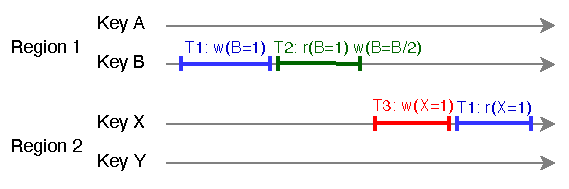
\includegraphics[width=0.63\columnwidth]{figures/RLS_SS.pdf}
    }
	\hfill
    \subfloat[\footnotesize Allowed by RSS but disallowed by \xxcons.\label{fig:rls_rss}]{
        \centering
        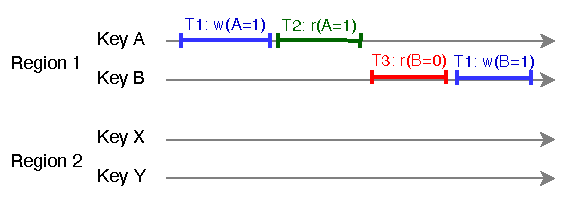
\includegraphics[width=0.63\columnwidth]{figures/RLS_RSS}
    }
    \hfill
    \subfloat[\footnotesize Allowed by \crdb but disallowed by \xxcons\label{fig:rls_crdb}]{
        \centering
         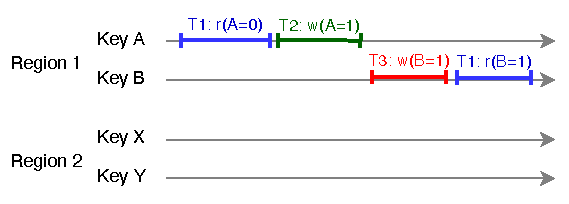
\includegraphics[width=0.63\columnwidth]{figures/RLS_CRDB.pdf}
    }
	\caption{Comparison of \xxcons with proximal levels of consistency models.}
\end{figure*}

\section{Related Works}\label{sec:related}
Transaction processing represents a well-explored area of research, with a plethora of influential works. We will provide an overview of related works in this section.

\subsection{Proximal Consistency Models}\label{sec:rls:compare}

\fig{fig:model} compares RLS to its proximal consistency models. We describe three of them in detail. All of them are serializable.

\begin{figure}[t]  
    \centering
    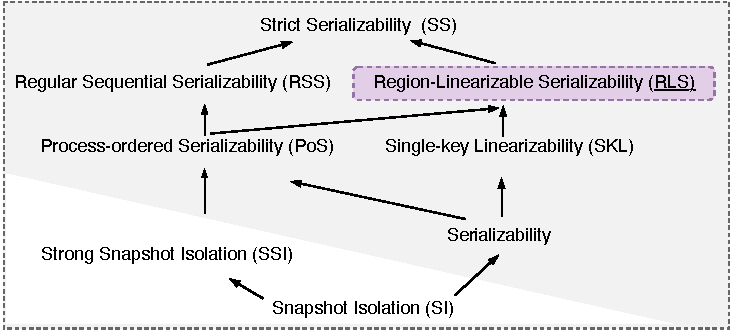
\includegraphics[width=\columnwidth]{figures/model.pdf}
  % \vspace{-5pt}
    \caption{This diagram shows how RLS compared to its proximal consistency models: SS~\cite{papadimitriou1979serializability}, RSS~\cite{rss}, SKL~\cite{taft2020cockroachdb}, PoS~\cite{daudjee2004lazy, lu2016snow}, SSI~\cite{fekete2005making}, serializability~\cite{viotti2016consistency}, and SI~\cite{anderson1998replication}. We highlight all those serializable consistency models in grey.} \label{fig:model}
  \end{figure}

\noindent\textbf{Regular Sequential Serializability (RSS)} complements \xxcons, as they focus on different aspects of distributed databases. RSS is primarily tailored for read-only transactions, permitting two read-only transactions to observe partial results of a committed read-write transaction in arbitrary orders (see our example in \fig{fig:rls_rss}). This behavior essentially violates the real-time ordering among read-only transactions.
On the contrary, \xxcons focuses on data locality within multi-region deployments, allowing a database system to relax the real-time ordering among transactions that access non-interleaved regions (refer to \fig{fig:rls_ss}). 
As illustrated in \fig{fig:rls_rss}, RSS allows transaction $T_2$ to read the writes made by a concurrent transaction $T_1$, while $T_3$ following $T_2$ reads a version preceding $T_1$. Consequently, the real-time order between $T_2$ and $T_3$ is disrupted: the real-time order between $T_2$ and $T_3$ is $T_2 \rightarrow T_3$; the serializable order enforced by RSS is $T_3 \rightarrow T_1 \rightarrow T_2$, which implies $T_3 \rightarrow T_2$.
This execution is not allowed by \xxcons since RLS ensures strict serializability (i.e., real-time order) for IRTs within the same region. 
% On the flip side, the execution shown in \fig{fig:rls_ss} is allowed by \xxcons but disallowed by RSS.

\noindent\textbf{Single-key Linearizability (SKL)} was initially proposed by CockroachDB~\cite{taft2020cockroachdb}. SKL stands as a strictly weaker variant of \xxcons. Like RLS, SKL guarantees serializability and ``no stale-reads''. However, unlike RLS, SKL does not preserve real-time orders between non-conflicting transactions. For instance, the execution illustrated in \fig{fig:rls_crdb} is permissible by SKL since there are ``no stale reads'' for each accessed key. However, it violates the real-time ordering between $T_2$ and $T_3$ in the same region, as the serial order is $T_3 \rightarrow T_1 \rightarrow T_2$, a violation not allowed by \xxcons. While weaker SKL may suffice for certain applications, other applications might necessitate stronger guarantees. Moreover, preventing consistency anomalies can significantly streamline application development.


\noindent\textbf{Process-ordered Serializability (PoS)} complements \xxcons. In a real deployment scenario, \xxcons can be stronger than PoS by associating each client with its nearby region. Specifically, PoS tracks the causal relations of each client and ensures the system preserves the ordering within each client's requests. If each client is associated with a region (e.g., sending requests to nodes within its region), \xxcons can prove to be strictly stronger than PoS since it guarantees real-time ordering for each client. 


\subsection{Transaction Priority}\label{sec:related:priority}

Compared to strict serializability (SS), one of the pivotal innovations of RLS is scheduling IRTs ahead of CRTs until the CRTs' order is established. Therefore, RLS operates under the assumption that IRTs have a higher priority than CRTs until CRTs have been ordered, after which both IRTs and CRTs are given equal priority for execution.

In this context, multi-region database developers can leverage existing transaction priority protocols to transition from SS to RLS, enhancing performance. For instance, Polaris~\cite{ye2023polaris} represents a transaction priority protocol rooted in a variant of OCC. Polaris embeds priority-related conflict detection within each record and permits priority preemption during runtime. 
Furthermore, Polaris avoids global operations, mitigating substantial overhead in a multi-region deployment. Consequently, achieving RLS should involve drawing inspiration from OCC-like concurrency control protocols. 

\subsection{Mixed Consistency Models}\label{sec:related:mixed}
Several prior works~\cite{milano2018mixt, li2012making, wang2021autogr, yang2017hierarchical, li2018fine, gao2003application, kraska2009consistency, mdcc:eurosys13} have been on manipulating weakly and strongly consistent transactions within a single database. For instance, MixT~\cite{milano2018mixt} advocates that consistency is a property of information. It proposes a new embedded language enabling users to configure the consistency guarantees for each operation manually. Similarly, Red-Blue consistency~\cite{li2012making} allows strongly and causally consistent operations to co-exist in a single system in the transaction's granularity and depends on application semantics to make ``consistency choices''. AutoGR~\cite{wang2021autogr} automatically analyzes and identifies the minimal set of the required consistency guarantees based on applications using the Z3 theorem prover. However, it relies on the application codes as inputs and only provides serializable guarantees without real-time order.

In contrast, RLS is geared towards multi-region deployments, directly integrating network semantics into the consistency model. Consequently, RLS does not depend on prior application knowledge to manually set distinct consistency guarantees for different transactions or operations. Moreover, RLS provides serializability (i.e., the strongest isolation levels) for all transactions while tailoring real-time properties to achieve heightened performance.